\section{Introduction}

Scientific publishing requires standardized document formatting and consistent presentation to effectively communicate research findings. LaTeX has emerged as the gold standard for academic document preparation, offering precise control over typography, mathematics, and figure placement. However, creating publication-ready documents from scratch can be time-consuming and technically challenging for researchers who prefer to focus on content rather than formatting.

Template engines address this challenge by providing pre-configured document structures that combine best practices in typography with field-specific requirements. The HenriquesLab style, originally developed for biomedical publications, represents a sophisticated approach to scientific document formatting that emphasizes clarity, professional presentation, and reproducible workflows.

Article-Forge builds upon this foundation by creating a comprehensive template ecosystem that includes not only the LaTeX style files but also the complete infrastructure needed for modern scientific publishing. This includes automated build systems, figure management, bibliography integration, and continuous documentation. The template is designed to be self-documenting, serving both as a publication tool and as an example of its own capabilities.

The development of robust scientific computing tools, such as NanoPyX \cite{nanopyx2024}, demonstrates the importance of well-documented, accessible software in advancing research. Similarly, Article-Forge aims to democratize access to professional document preparation by removing technical barriers while maintaining the highest standards of academic presentation.

Modern scientific workflows increasingly require reproducible, automated processes that can be easily shared and adapted across research groups. Article-Forge addresses these needs by providing a complete template engine that can be version-controlled, customized, and deployed across different computing environments. The template includes containerization support, automated testing, and comprehensive documentation to ensure reliability and ease of use.

You can include figures like Figure~\ref{fig:example} to demonstrate template capabilities and document structure.

\begin{figure}[htbp]
    \centering
    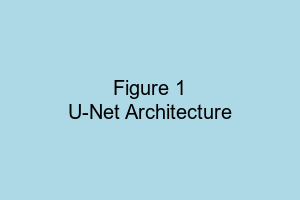
\includegraphics[width=0.8\textwidth]{Figure1.png}
    \caption{Overview of the Article-Forge template structure and workflow. This diagram illustrates the components of the template engine, from source files and style sheets to automated build processes and final PDF generation.}
    \label{fig:example}
\end{figure}

This article demonstrates the capabilities of Article-Forge by using the template to document itself, providing a practical example of how researchers can leverage this tool for their own publications.
